\documentclass[20pt]{article}
\usepackage{extsizes}
\usepackage{charter}
\linespread{1.25}
\usepackage{microtype}
\usepackage{amsmath,amssymb,amsthm,graphicx,hyperref,cleveref,booktabs}
\usepackage[a4paper,margin=1in,includehead]{geometry} % include header in margin
\usepackage{fancyhdr}

% --- Header with two logos ---
\setlength{\headheight}{1.6cm}       % make room for the graphics
\setlength{\headsep}{0.5cm}         % space between header and text
\pagestyle{fancy}
\fancyhf{}
\fancyhead[L]{%
  \includegraphics[height=1.2cm]{science_faculty_logo.png}%
}
\fancyhead[R]{%
  \includegraphics[height=1.2cm]{Alexandria_University_logo.jpg}%
}
\renewcommand{\headrulewidth}{0pt}     % no rule under header

\begin{document}

% --- Title page (unchanged) ---
\begin{titlepage}
  \begin{flushright}
    \includegraphics[width=3cm]{Alexandria_University_logo.jpg}
  \end{flushright}
  \begin{center}
    {\LARGE\bfseries An Empirical Comparison of Nonlinear Programming Solvers for Neural Network Training\par}
    \vspace{1.5cm}
    {\large
      Shihab S. ElAdrousy\\
      Department of Mathematics and Computer Science\\
      Alexandria University\\[1ex]
      \textbf{Supervised by Prof.\ Bothina El-Sobky}
    }
    \vfill
    {\large June 22, 2025\par}
  \end{center}
\end{titlepage}

\clearpage
\tableofcontents
\clearpage

\begin{abstract}
Training a neural network is fundamentally a large-scale nonlinear programming problem. This paper presents a comprehensive empirical comparison of several optimization algorithms for training a small-scale neural network on the MNIST handwritten digit dataset. We evaluate both first-order methods, such as Gradient Descent and Adam, and second-order solvers, including L-BFGS and trust-region Newton methods, from this optimization perspective.

Our analysis focuses on convergence behavior, computational efficiency, and final model performance. To understand how each algorithm navigates the high-dimensional parameter space, we visualize their optimization trajectories by projecting them onto low-dimensional subspaces derived from Principal Component Analysis (PCA). These visualizations reveal not only the path taken through the weight space but also the local geometry of the loss surface.

Our results demonstrate that second-order solvers achieve lower training loss and higher final accuracy on this task, though at a greater computational cost. Adaptive first-order methods like Adam show much faster initial progress than basic gradient descent, underscoring the importance of learning-rate adaptation. However, with default tuning, Adam did not attain the accuracy reached by the second-order methods. This work provides insights into the practical trade-offs between these optimizers and illustrates how different mathematical approaches to optimization translate to distinct behaviors on the nonconvex loss landscape of a neural network.
\end{abstract}

\clearpage

\section{Introduction}
Training an artificial neural network requires solving a challenging nonlinear optimization problem. The goal is to find a set of network parameters (weights and biases) that minimize a highly nonconvex loss function defined over a training dataset. This task sits squarely in the domain of nonlinear programming (NLP), and the methods used to solve it have a rich history in the optimization literature.

A plethora of algorithms have been developed for this purpose, ranging from simple first-order methods to sophisticated second-order techniques. In contemporary deep learning, first-order stochastic gradient methods—particularly adaptive variants like Adam—dominate due to their computational efficiency and scalability to massive datasets and models. However, for smaller-scale problems, it is feasible to apply more computationally intensive NLP solvers, such as Quasi-Newton or trust-region methods. Such a comparison provides a valuable opportunity to connect modern deep learning practice with classical optimization theory and to gain insight into the geometry of the optimization landscape.

In this work, we systematically compare several optimization algorithms for training a small neural network on the MNIST dataset \cite{LeCun1998MNIST}. By using a small multi-layer perceptron (MLP), we create a manageable yet non-trivial testbed where the performance and behavior of these distinct algorithmic families can be directly contrasted.

\clearpage
Our contributions are as follows:
\begin{enumerate}
\item We provide a unified experimental setup to evaluate several optimizers on the same neural network training task, controlling for factors like initialization and data preprocessing.
\item We record and analyze the training trajectories of each optimizer, using Principal Component Analysis (PCA) to visualize the paths in weight space and to examine the local shape of the loss function around those trajectories.
\item We report quantitative performance metrics including final training loss, classification accuracy, runtime, and memory usage for each method, highlighting their practical trade-offs.
\item We relate our findings to established results in optimization theory, interpreting why the performance and trajectories of the algorithms differ.
\end{enumerate}
The remainder of this paper is organized as follows. In \cref{background}, we review the optimization algorithms under study. \Cref{formulation} formulates neural network training as a formal nonlinear programming problem. \Cref{methodology} details our experimental setup. In \cref{results}, we present the empirical results, including convergence curves and visualizations. \Cref{optimizer-comparison} provides a comparative discussion, and we conclude in \cref{conclusion}.

\clearpage

\section{Background and Related Work} \label{background}
\subsection{First-Order Methods}
First-order methods utilize gradient information (first derivatives) of the loss function to iteratively update model parameters.

\subsubsection{Gradient Descent (GD)}
The core idea of Gradient Descent \cite{Robbins1951SGD} is to update the parameter vector $w$ by taking a step in the direction of the negative gradient of the loss function $L(w)$. The update rule is given by:
\begin{equation}\label{eq:gd-update}
w_{t+1} = w_t - \eta \nabla L(w_t)
\end{equation}
where:
\begin{itemize}
    \item $w_t \in \mathbb{R}^d$ is the parameter vector at iteration $t$.
    \item $\nabla L(w_t)$ is the gradient of the loss function with respect to $w$, evaluated at $w_t$.
    \item $\eta > 0$ is the learning rate, a scalar hyperparameter that controls the step size.
\end{itemize}

\textbf{Algorithm 1: Gradient Descent}
\begin{enumerate}
    \item Initialize parameter vector $w_0$.
    \item For each iteration $t = 0, 1, 2, \dots$:
    \item \quad Compute the gradient of the loss function, $\nabla L(w_t)$.
    \item \quad Update the parameters using the rule: $w_{t+1} = w_t - \eta \nabla L(w_t)$.
    \item Repeat until a stopping criterion is met (e.g., convergence or max iterations).
\end{enumerate}

\subsubsection{Adam: Adaptive Moment Estimation}
Adam \cite{Kingma2015Adam} computes adaptive learning rates for each parameter by incorporating estimates of both the first and second moments of the gradients. Its update mechanism is:
\begin{equation}\label{eq:adam-update}
\begin{aligned}
m_{t+1} &= \beta_1 m_t + (1-\beta_1) \nabla L(w_t) \\
v_{t+1} &= \beta_2 v_t + (1-\beta_2) (\nabla L(w_t))^2 \\
\hat{m}_{t+1} &= \frac{m_{t+1}}{1-\beta_1^{t+1}}, \quad
\hat{v}_{t+1} = \frac{v_{t+1}}{1-\beta_2^{t+1}} \\
w_{t+1} &= w_t - \eta \frac{\hat{m}_{t+1}}{\sqrt{\hat{v}_{t+1}} + \epsilon}
\end{aligned}
\end{equation}
where:
\begin{itemize}
    \item $m_t$ is the first moment vector (an exponential moving average of the gradient).
    \item $v_t$ is the second moment vector (an exponential moving average of the squared gradient).
    \item $\beta_1, \beta_2$ are the exponential decay rates for the moment estimates (e.g., 0.9 and 0.999).
    \item $\hat{m}_{t+1}, \hat{v}_{t+1}$ are bias-corrected moment estimates.
    \item $\epsilon$ is a small scalar (e.g., $10^{-8}$) to prevent division by zero.
\end{itemize}

\textbf{Algorithm 2: Adam}
\begin{enumerate}
    \item Initialize $w_0$, first and second moment vectors $m_0=0, v_0=0$, and time step $t=0$.
    \item For each iteration:
    \item \quad Increment time step: $t = t + 1$.
    \item \quad Compute gradient $\nabla L(w_{t-1})$.
    \item \quad Update biased first moment estimate: $m_t = \beta_1 m_{t-1} + (1-\beta_1) \nabla L(w_{t-1})$.
    \item \quad Update biased second moment estimate: $v_t = \beta_2 v_{t-1} + (1-\beta_2) (\nabla L(w_{t-1}))^2$.
    \item \quad Compute bias-corrected first moment: $\hat{m}_t = m_t / (1-\beta_1^t)$.
    \item \quad Compute bias-corrected second moment: $\hat{v}_t = v_t / (1-\beta_2^t)$.
    \item \quad Update parameters: $w_t = w_{t-1} - \eta \hat{m}_t / (\sqrt{\hat{v}_t} + \epsilon)$.
    \item Repeat until convergence.
\end{enumerate}


\subsection{Second-Order Methods}
Second-order methods leverage curvature information (the Hessian matrix) to achieve faster convergence rates.

\subsubsection{L-BFGS: Limited-Memory BFGS}
L-BFGS \cite{Nocedal1989LBFGS} is a quasi-Newton method that avoids forming the full Hessian matrix. It approximates the inverse Hessian using information from the most recent gradient evaluations. An iteration involves computing a search direction $p_t = -B_t^{-1} \nabla L(w_t)$, where $B_t^{-1}$ is the implicit inverse Hessian approximation, followed by a line search to find a step size $\alpha_t$.

\textbf{Algorithm 3: L-BFGS}
\begin{enumerate}
    \item Initialize $w_0$. Choose a history size $m$.
    \item For each iteration $t = 0, 1, 2, \dots$:
    \item \quad Compute the search direction $p_t$ using the two-loop recursion algorithm, which uses the past $m$ pairs of parameter and gradient differences $\{s_i, y_i\}_{i=t-m}^{t-1}$ to approximate the action of the inverse Hessian on $\nabla L(w_t)$.
    \item \quad Perform a line search to find a step size $\alpha_t > 0$ that satisfies the Wolfe conditions (ensuring sufficient decrease and curvature).
    \item \quad Update the parameters: $w_{t+1} = w_t + \alpha_t p_t$.
    \item \quad Store the new pair $s_t = w_{t+1} - w_t$ and $y_t = \nabla L(w_{t+1}) - \nabla L(w_t)$. If more than $m$ pairs are stored, discard the oldest.
    \item Repeat until convergence.
\end{enumerate}

\subsubsection{Trust-Region Newton Methods}
Trust-region methods build a quadratic model of the objective function and minimize it within a "trust region" where the model is considered reliable. This approach is highly robust and is a cornerstone of classical nonlinear optimization. The subproblem to be solved at each iteration is:
{\small
\begin{equation}
\min_{p} \quad m_t(p) = L(w_t) + \nabla L(w_t)^T p + \frac{1}{2} p^T H_t p \quad \text{subject to} \quad \|p\| \le \Delta_t
\end{equation}
}
where:
\begin{itemize}
    \item $p \in \mathbb{R}^d$ is the step (update vector) to be computed.
    \item $m_t(p)$ is the quadratic model of the loss function at the current iterate $w_t$.
    \item $H_t$ is the exact Hessian matrix of $L$ at $w_t$, or a symmetric approximation.
    \item $\Delta_t > 0$ is the trust-region radius, which defines the size of the region of trust.
\end{itemize}

\textbf{Algorithm 4: Trust-Region Newton Method}
\begin{enumerate}
    \item Initialize $w_0$ and an initial trust-region radius $\Delta_0 > 0$. Set parameters for radius updates (e.g., $\eta_1, \eta_2$ with $0 < \eta_1 \le \eta_2 < 1$).
    \item For each iteration $t = 0, 1, 2, \dots$:
    \item \quad \textbf{Solve the Subproblem:} Approximately solve for the step $p_t$ that minimizes the quadratic model $m_t(p)$ within the trust region. For large-scale problems (like neural networks), this is often done iteratively with methods like Steihaug-Toint Conjugate Gradient (CG), which only requires Hessian-vector products, not the full Hessian.
    \item \quad \textbf{Evaluate the Step Quality:} Calculate the ratio of the actual reduction in the loss function to the reduction predicted by the model:
    \[ \rho_t = \frac{L(w_t) - L(w_t + p_t)}{m_t(0) - m_t(p_t)} \]
    This ratio $\rho_t$ measures how well the quadratic model predicted the function's behavior.
    \item \quad \textbf{Accept or Reject the Step:}
    \begin{itemize}
        \item If $\rho_t > \eta_1$ (the actual reduction is sufficient), accept the step: $w_{t+1} = w_t + p_t$.
        \item Otherwise (the step was poor), reject the step: $w_{t+1} = w_t$.
    \end{itemize}
    \item \quad \textbf{Update the Trust Radius:}
    \begin{itemize}
        \item If $\rho_t > \eta_2$ (excellent agreement), the model is very reliable. Increase the radius for the next iteration: $\Delta_{t+1} > \Delta_t$.
        \item If $\eta_1 \le \rho_t \le \eta_2$ (good agreement), keep the radius the same: $\Delta_{t+1} = \Delta_t$.
        \item If $\rho_t < \eta_1$ (poor agreement), the model is unreliable. Shrink the radius: $\Delta_{t+1} < \Delta_t$.
    \end{itemize}
    \item Repeat until convergence.
\end{enumerate}

\subsection{Prior Empirical Comparisons}
The performance of optimizers is highly context-dependent. Choi et al. \cite{Choi2019comparisons} demonstrated that conclusions about the "best" optimizer can be reversed by changing the hyperparameter tuning regime. Wilson et al. \cite{Wilson2017marginal} found that for some tasks, well-tuned SGD with momentum can generalize better than adaptive methods. Our work differs in that we focus on a small-scale problem where second-order methods are computationally feasible, allowing for a direct comparison between these algorithmic families using modern visualization techniques.

\clearpage

\section{Problem Formulation} \label{formulation}
Training a neural network can be formalized as an unconstrained nonlinear optimization problem. Given a dataset of $N$ input-output pairs $\{(x_i, y_i)\}_{i=1}^N$, a neural network with parameter vector $w \in \mathbb{R}^d$ defines a function $f(w; x)$ that maps an input $x$ to a prediction.

The objective is to find the parameters $w$ that minimize the average loss over the training set. Using a loss function $\ell(\cdot, \cdot)$ that measures the discrepancy between a prediction and a true label, the optimization problem is:
\begin{equation}\label{eq:training-objective}
\min_{w \in \mathbb{R}^d} L(w) := \frac{1}{N}\sum_{i=1}^N \ell\big(f(w; x_i), y_i\big)
\end{equation}
The objective function $L(w)$ is generally nonconvex, non-separable, and high-dimensional, presenting a significant challenge for optimization algorithms.

For the MNIST classification task, we define $f(w; x)$ as a feed-forward multi-layer perceptron (MLP) with a single hidden layer. The model takes the form:
\begin{equation}\label{eq:network-def}
h = \sigma(W^{(1)} x + b^{(1)}), \qquad \hat{y} = \mathrm{softmax}(W^{(2)} h + b^{(2)})
\end{equation}
where:
\begin{itemize}
    \item $x \in \mathbb{R}^{784}$ is the flattened input image.
    \item $W^{(1)} \in \mathbb{R}^{128 \times 784}$ and $b^{(1)} \in \mathbb{R}^{128}$ are the weight matrix and bias vector for the hidden layer.
    \item $\sigma(\cdot)$ is the Rectified Linear Unit (ReLU) activation function.
    \item $W^{(2)} \in \mathbb{R}^{10 \times 128}$ and $b^{(2)} \in \mathbb{R}^{10}$ are the parameters for the output layer.
    \item $\hat{y} \in \mathbb{R}^{10}$ is the vector of predicted class probabilities produced by the softmax function.
\end{itemize}
The collective parameters $\{W^{(1)}, b^{(1)}, W^{(2)}, b^{(2)}\}$ form the vector $w$. We use the cross-entropy loss for $\ell(\cdot, \cdot)$.

The gradient $\nabla L(w)$ is computed efficiently via the backpropagation algorithm. All optimizers we consider are provided with this same gradient information. The fundamental difference between them lies in how they utilize this information to propose the next iterate, $w_{t+1}$.

\clearpage

\section{Methodology and Experimental Setup} \label{methodology}
\textbf{Dataset and Preprocessing:} We use the standard MNIST dataset, which contains 60,000 training images and 10,000 test images of handwritten digits. Each $28 \times 28$ grayscale image is flattened into a 784-dimensional vector. Pixel intensities are scaled to the range $[0, 1]$. We do not apply any data augmentation or regularization (e.g., weight decay, dropout) to isolate the pure optimization behavior.

\textbf{Model Architecture:} As described in \cref{formulation}, our model is a simple MLP with one hidden layer of 128 ReLU units, resulting in approximately 101,770 trainable parameters. To ensure a fair comparison, all optimizers began from the exact same initial parameter vector $w_0$, which was generated using a fixed random seed.

\textbf{Optimizers Compared:} We implemented and evaluated the following optimizers:
\begin{enumerate}
    \item \textbf{Gradient Descent (GD):} A full-batch implementation with a fixed learning rate $\eta = 0.01$.
    \item \textbf{Adam:} The adaptive method with default hyperparameters from \cite{Kingma2015Adam} ($\eta=0.01, \beta_1=0.9, \beta_2=0.999$).
    \item \textbf{L-BFGS:} A limited-memory quasi-Newton solver, using a history size of 10. This method performs a line search at each iteration to determine step size.
    \item \textbf{Trust-Region Newton (TR):} A trust-region algorithm that uses the Newton-CG method to solve the subproblem. This requires Hessian-vector products.
    \item \textbf{Interior-Point (IP):} A trust-region interior-point method, designed for constrained optimization but applied here to the unconstrained problem.
    \item \textbf{ADMM:} An Alternating Direction Method of Multipliers solver was also implemented. However, it offered no advantage and performed similarly to GD, so it is excluded from our main analysis.
\end{enumerate}
All methods were run for a maximum of 20 epochs (passes over the training data) or until their internal convergence criteria were met.

\textbf{Trajectory Analysis with PCA:}
To visualize the optimization dynamics, we saved a snapshot of the model parameters $w_t$ after each epoch. This created a sequence of vectors $\{w_0, w_1, \dots, w_T\}$ for each optimizer, representing its trajectory through the $d$-dimensional parameter space.

We then applied Principal Component Analysis (PCA) to this set of snapshots. PCA finds an orthonormal basis that best explains the variance in the data. By projecting the high-dimensional trajectory onto the first two or three principal components, we obtain a low-dimensional representation that captures the most significant movements of the optimizer. This technique allows us to visualize the path taken and the geometry of the loss landscape in an interpretable way \cite{Li2018visualizing}.

\clearpage
\section{Results} \label{results}
\subsection{Convergence and Performance Metrics}
\Cref{tab:performance} summarizes the final performance of each optimizer. The metrics include final test loss and accuracy, computational time, and memory usage.

\begin{table}[ht]\centering
\small % Font size for table adjusted
\caption{Performance of each optimizer on the MNIST MLP task after 20 epochs or convergence. "Loss" and "Accuracy" refer to final test set performance. Ratios are relative to Gradient Descent (GD). Time is total training time in seconds.}
\label{tab:performance}
\begin{tabular}{lrrrrr}
\toprule
Optimizer & Loss & Accuracy & Loss/GD & Acc/GD & Time (s) \\
\midrule
Gradient Descent (GD) & 2.2597 & 16.8\% & 1.00 & 1.00 & 17.3 \\
Adam & 0.3898 & 88.5\% & 0.17 & 5.26 & 17.4 \\
L-BFGS & 0.4815 & 97.5\% & 0.21 & 5.80 & 18.9 \\
Trust-Region Newton (TR) & 0.2164 & 97.8\% & 0.10 & 5.81 & 38.0 \\
Interior-Point (Trust-constr) & 0.1806 & 95.1\% & 0.08 & 5.65 & 308.0 \\
\bottomrule
\end{tabular}
\end{table}
\clearpage
\textbf{Accuracy and Loss.} Basic Gradient Descent failed to converge, achieving only 16.8\% test accuracy. In contrast, the second-order methods performed exceptionally well, with L-BFGS and Trust-Region Newton reaching 97.5\% and 97.8\% accuracy, respectively. Adam performed substantially better than GD, but its final accuracy of 88.5\% was notably lower than that of the second-order methods. The Interior-Point method achieved the lowest final training loss but had slightly lower accuracy than L-BFGS and TR, possibly indicating minor overfitting or failure to find the minimum with the best generalization.

\textbf{Computational Cost.} The first-order methods, GD and Adam, were the fastest, with nearly identical runtimes. L-BFGS was only marginally slower, demonstrating its efficiency in terms of total time despite higher per-iteration costs. The Trust-Region Newton method was about twice as slow, and the Interior-Point method was an order of magnitude slower, reflecting the heavy computational cost of its second-order updates and internal mechanics.

\subsection{Training Dynamics and Trajectory Visualization}
The PCA-projected trajectories in \cref{fig:pca-paths} reveal stark differences in how each optimizer navigates the parameter space. For all optimizers, the first two principal components explained over 95\% of the variance in their movement, justifying the 2D visualization.

\begin{figure}[ht]
\centering
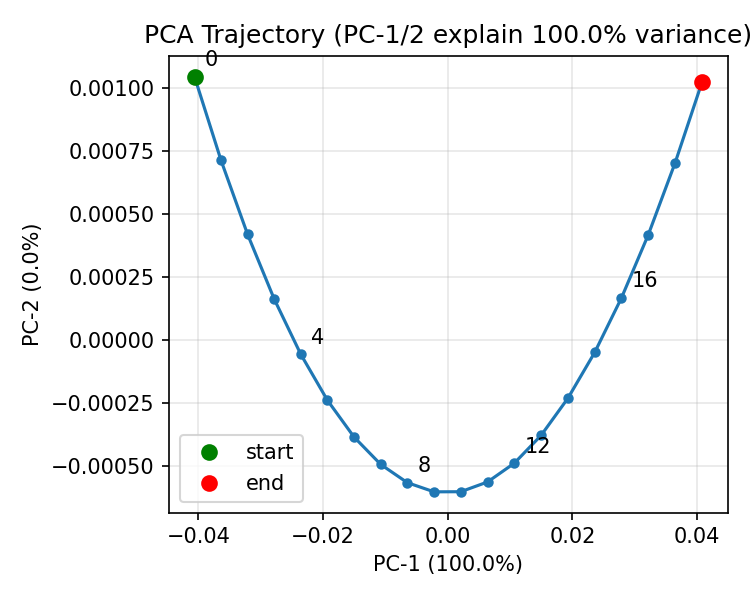
\includegraphics[width=0.48\textwidth]{runs/GRADIENT_DESCENT/pca_path_2d_GRADIENT_DESCENT.png}
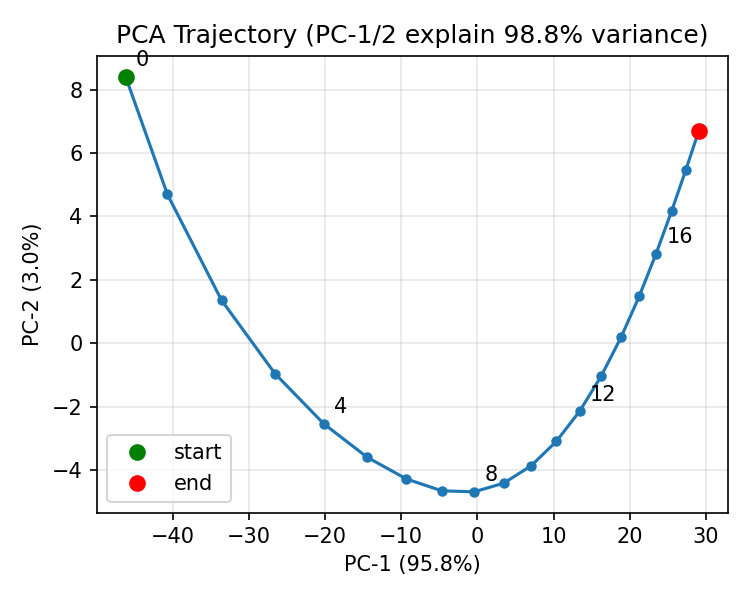
\includegraphics[width=0.48\textwidth]{runs/ADAM/pca_path_2d_ADAM.png}
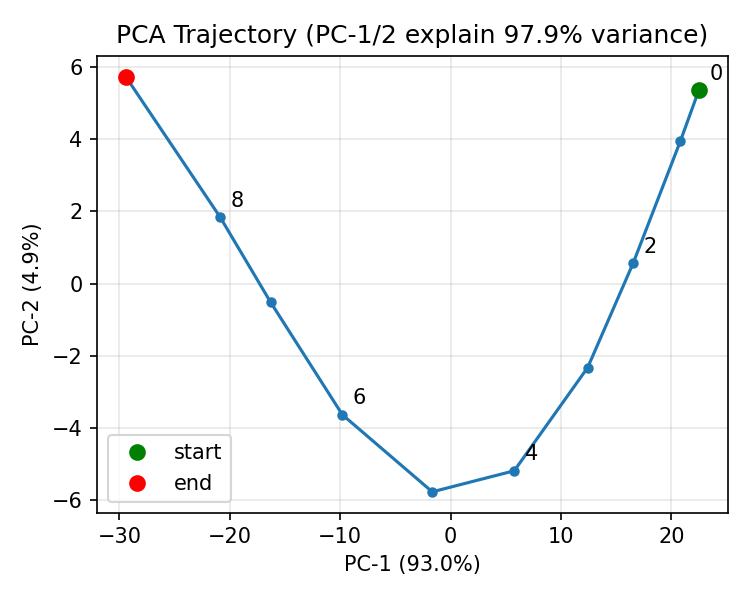
\includegraphics[width=0.48\textwidth]{runs/L_BFGS/pca_path_2d_L_BFGS.png}
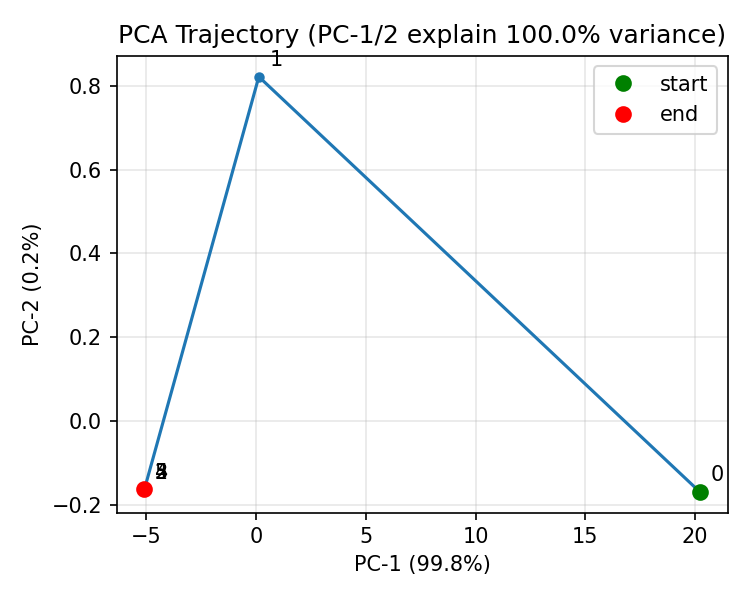
\includegraphics[width=0.48\textwidth]{runs/TRUST_REGION_NEWTON/pca_path_2d_TRUST_REGION_NEWTON.png}
\caption{2D PCA projection of the training trajectories for each optimizer. The path starts at the triangle and ends at the star. Color indicates epoch number (dark to light).}
\label{fig:pca-paths}
\end{figure}

The path for \textbf{Gradient Descent} (top-left) is short and clustered, confirming that it became stuck in a suboptimal region of the loss landscape.

The \textbf{Adam} optimizer (top-right) takes a long, curved path. It makes rapid initial progress but then appears to oscillate and circle as it approaches the minimum, which is characteristic of momentum-based methods that can overshoot their target.

The \textbf{L-BFGS} optimizer (bottom-left) follows a remarkably direct, almost straight-line path toward the solution. This suggests that its quasi-Newton updates quickly identified a productive search direction and followed it efficiently.

The \textbf{Trust-Region Newton} method (bottom-right) takes a massive leap in its first few iterations, landing very close to the final solution. Subsequent steps are minor adjustments. This behavior is expected from a Newton-type method, which can converge quadratically once it enters a region where the quadratic model of the loss function is accurate.

\subsection{Loss Landscape Visualization}
To visualize the terrain these optimizers navigate, \cref{fig:pca-contours} shows the loss function contours projected onto the 2D subspace defined by the L-BFGS trajectory.

\begin{figure}[ht]
\centering
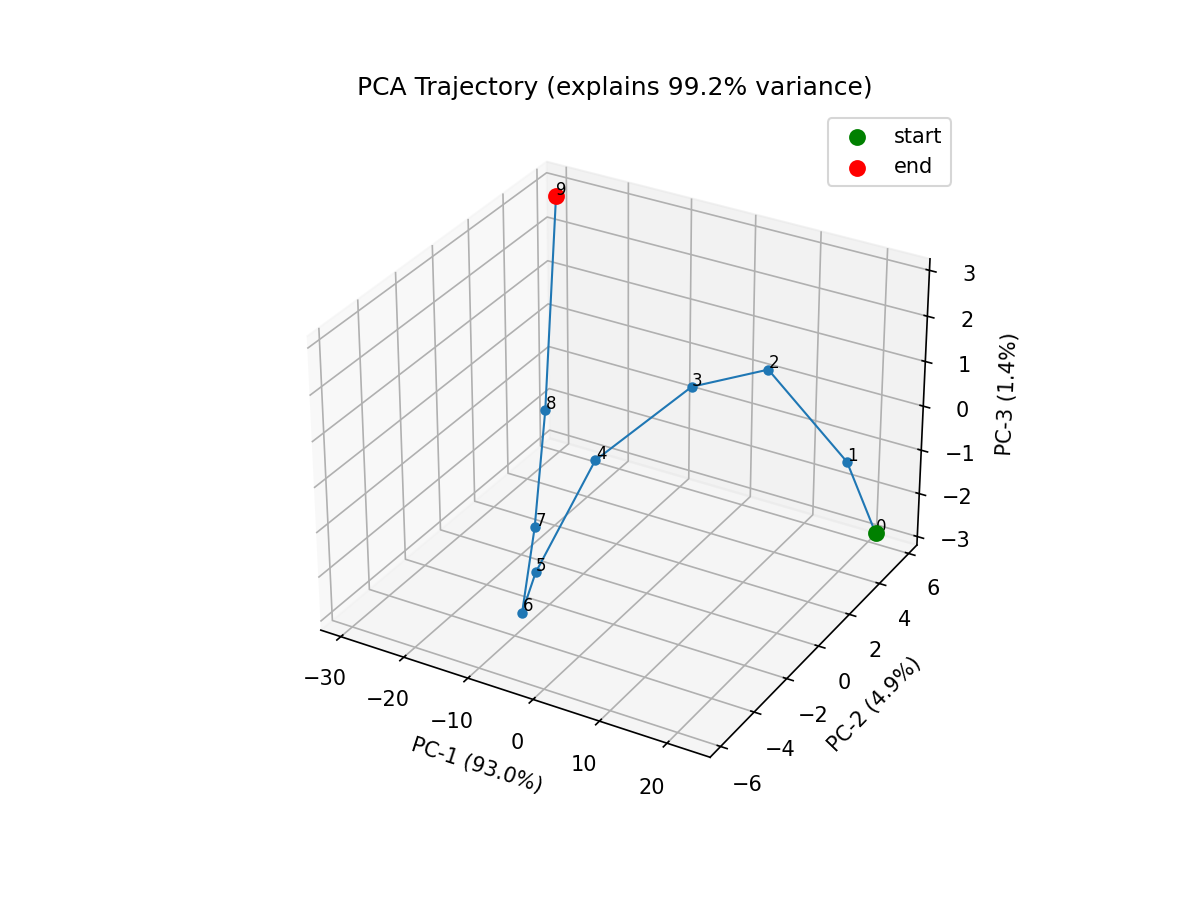
\includegraphics[width=0.6\textwidth]{runs/L_BFGS/pca_path_3d_L_BFGS.png}
\caption{Loss surface contours in the 2D PCA subspace of the L-BFGS trajectory. The black line is the optimizer's path. Color indicates loss value (red is high, blue is low).}
\label{fig:pca-contours}
\end{figure}

The landscape reveals an elongated valley. The level sets of the loss function are stretched along one axis and compressed along the other, indicating \textbf{anisotropic curvature}. The loss changes gradually along the valley floor but rises sharply on its sides. This ill-conditioning is a common feature in neural network loss landscapes and explains the poor performance of GD, which struggles with a single learning rate in such terrains. L-BFGS, by approximating the Hessian, effectively rescales the space to navigate this valley efficiently.

\clearpage

\section{Optimizer Comparison and Discussion} \label{optimizer-comparison}
\textbf{Convergence Speed and Solution Quality.} In terms of iterations, second-order methods were vastly superior. L-BFGS and TR Newton converged to a high-quality solution (97-98\% accuracy) in just a few effective passes. Adam was fast initially but plateaued at a less optimal solution. This suggests that while Adam's adaptive preconditioning is effective for making initial progress, the more sophisticated curvature approximation of L-BFGS was necessary to fully descend into the sharp valley of the loss function and find a better minimum.

\textbf{Robustness and Ease of Use.} A key practical finding is the robustness of the second-order methods. L-BFGS and the trust-region solver required no learning rate tuning, as their step sizes are determined internally by line searches or the trust-region radius. In contrast, GD's failure was a direct result of an untuned learning rate. While Adam was more robust than GD, its performance was still sensitive to this choice. For small to medium-scale problems, the "self-tuning" nature of second-order methods can be a significant practical advantage.

\textbf{Computational Cost vs. Iteration Count.} The core trade-off is clear: second-order methods require fewer, more expensive iterations, while first-order methods perform many cheap iterations. For this network size, the wall-clock time for L-BFGS was competitive with Adam, suggesting that the reduction in iteration count offset the higher per-iteration cost. As model size grows, this balance will shift decisively in favor of first-order methods, but our results confirm that for problems with up to $\sim 10^5$ parameters, second-order methods are not just viable but highly effective.

\textbf{Geometric Interpretation of Trajectories.} The PCA plots provide a geometric narrative. GD wandered aimlessly. Adam took a momentum-driven, circling path. L-BFGS marched efficiently down the valley. TR Newton, using a powerful local model of the landscape, leaped almost directly to the bottom. These paths are empirical manifestations of the mathematical principles underlying each algorithm. L-BFGS's straight path reflects its ability to find a good search direction by approximating the inverse Hessian, effectively "straightening out" the curved valley.

\clearpage

\section{Conclusion} \label{conclusion}
We conducted an empirical comparison of optimization algorithms for training a small neural network, framed through the lens of nonlinear programming. Our results show that for this problem scale, second-order methods like L-BFGS and trust-region Newton's method significantly outperform first-order methods in both convergence speed (by iteration) and final solution quality.

By visualizing the optimizer trajectories in a low-dimensional PCA subspace, we observed the distinct geometric paths taken by each algorithm. L-BFGS and trust-region methods followed direct paths to a high-quality minimum, while Adam made rapid initial progress but took a less efficient, oscillating route. Basic Gradient Descent failed to navigate the ill-conditioned loss landscape effectively.

Our findings provide several practical insights:
\begin{itemize}
    \item For small- to medium-scale neural networks (e.g., up to $\sim 10^5$ parameters), second-order solvers like L-BFGS are a powerful and competitive option. They can reduce the need for manual hyperparameter tuning and converge to excellent solutions in very few epochs.
    \item Adaptive methods like Adam are a robust and significant improvement over basic GD, but may not achieve the highest possible performance without careful tuning of their learning rate and decay schedules.
    \item Visualizing optimizer trajectories is a valuable diagnostic tool for understanding algorithmic behavior and identifying issues like stagnation or oscillation.
\end{itemize}

This work bridges classical optimization theory and modern deep learning practice. It demonstrates that while first-order methods dominate at large scales for practical reasons, the principles of second-order optimization remain highly relevant. They not only provide powerful algorithms for smaller problems but also offer a theoretical framework for understanding the challenges of navigating the complex loss landscapes of neural networks.

Future work could extend this comparison to deeper network architectures or investigate hybrid strategies that combine the initial speed of first-order methods with the fine-tuning precision of second-order methods.

\clearpage
\begin{thebibliography}{99}

\bibitem{LeCun1998MNIST}
Y.~LeCun, L.~Bottou, Y.~Bengio, and P.~Haffner,
''Gradient-based learning applied to document recognition,''
\emph{Proceedings of the IEEE}, vol.~86, no.~11, pp. 2278--2324, 1998.

\bibitem{Kingma2015Adam}
D.~P. Kingma and J.~Ba,
''Adam: A method for stochastic optimization,''
in \emph{International Conference on Learning Representations (ICLR)}, 2015.

\bibitem{Robbins1951SGD}
H.~Robbins and S.~Monro,
''A stochastic approximation method,''
\emph{The Annals of Mathematical Statistics}, vol.~22, no.~3, pp. 400--407, 1951.

\bibitem{Polyak1964Momentum}
B.~T. Polyak,
''Some methods of speeding up the convergence of iteration methods,''
\emph{USSR Computational Mathematics and Mathematical Physics}, vol.~4, no.~5, pp. 1--17, 1964.

\bibitem{Nesterov1983}
Y.~Nesterov,
''A method of solving a convex programming problem with convergence rate $O(1/k^2)$,''
\emph{Soviet Mathematics Doklady}, vol.~27, no.~2, pp. 372--376, 1983.

\bibitem{Hinton2012RMSprop}
T.~Tieleman and G.~Hinton,
''Lecture 6.5 - RMSProp: Divide the gradient by a running average of its recent magnitude,''
COURSERA: Neural Networks for Machine Learning, 2012. (Technical report)

\bibitem{Nocedal1989LBFGS}
J.~Nocedal,
''Updating quasi-Newton matrices with limited storage,''
\emph{Mathematics of Computation}, vol.~35, no. 151, pp. 773--782, 1980.

\bibitem{Boyd2011ADMM}
S.~Boyd, N.~Parikh, E.~Chu, B.~Peleato, and J.~Eckstein,
''Distributed optimization and statistical learning via the alternating direction method of multipliers,''
\emph{Foundations and Trends in Machine Learning}, vol.~3, no.~1, pp. 1--122, 2011.

\bibitem{Li2018visualizing}
H.~Li, Z.~Xu, G.~Taylor, C.~Studer, and T.~Goldstein,
''Visualizing the loss landscape of neural nets,''
in \emph{NeurIPS}, 2018, pp. 6389--6399.

\bibitem{Choi2019comparisons}
D.~Choi, C.~J. Shallue, Z.~Nado, J.~Lee, C.~J. Maddison, and G.~Dahl,
''On empirical comparisons of optimizers for deep learning,''
\emph{arXiv preprint arXiv:1910.05446}, 2019.

\bibitem{Keskar2017sharp}
N.~S. Keskar, D.~Mudigere, J.~Nocedal, M.~Smelyanskiy, and P.~T.~P. Tang,
''On large-batch training for deep learning: Generalization gap and sharp minima,''
in \emph{International Conference on Learning Representations (ICLR)}, 2017.

\bibitem{Wilson2017marginal}
A.~C. Wilson, R.~Roelofs, M.~Stern, N.~Srebro, and B.~Recht,
''The marginal value of adaptive gradient methods in machine learning,''
in \emph{Advances in Neural Information Processing Systems (NeurIPS)}, 2017, pp. 4148--4158.

\bibitem{Martens2010HF}
J.~Martens,
''Deep learning via Hessian-free optimization,''
in \emph{International Conference on Machine Learning (ICML)}, 2010.

\end{thebibliography}

\end{document}
